\chapter{3D Vision}

\section{Image Formation}

The basic model is based on the principle of \textbf{camera obscura}, a room with a hole by which the light can enter the room.

\begin{figure}[H]
    \centering
    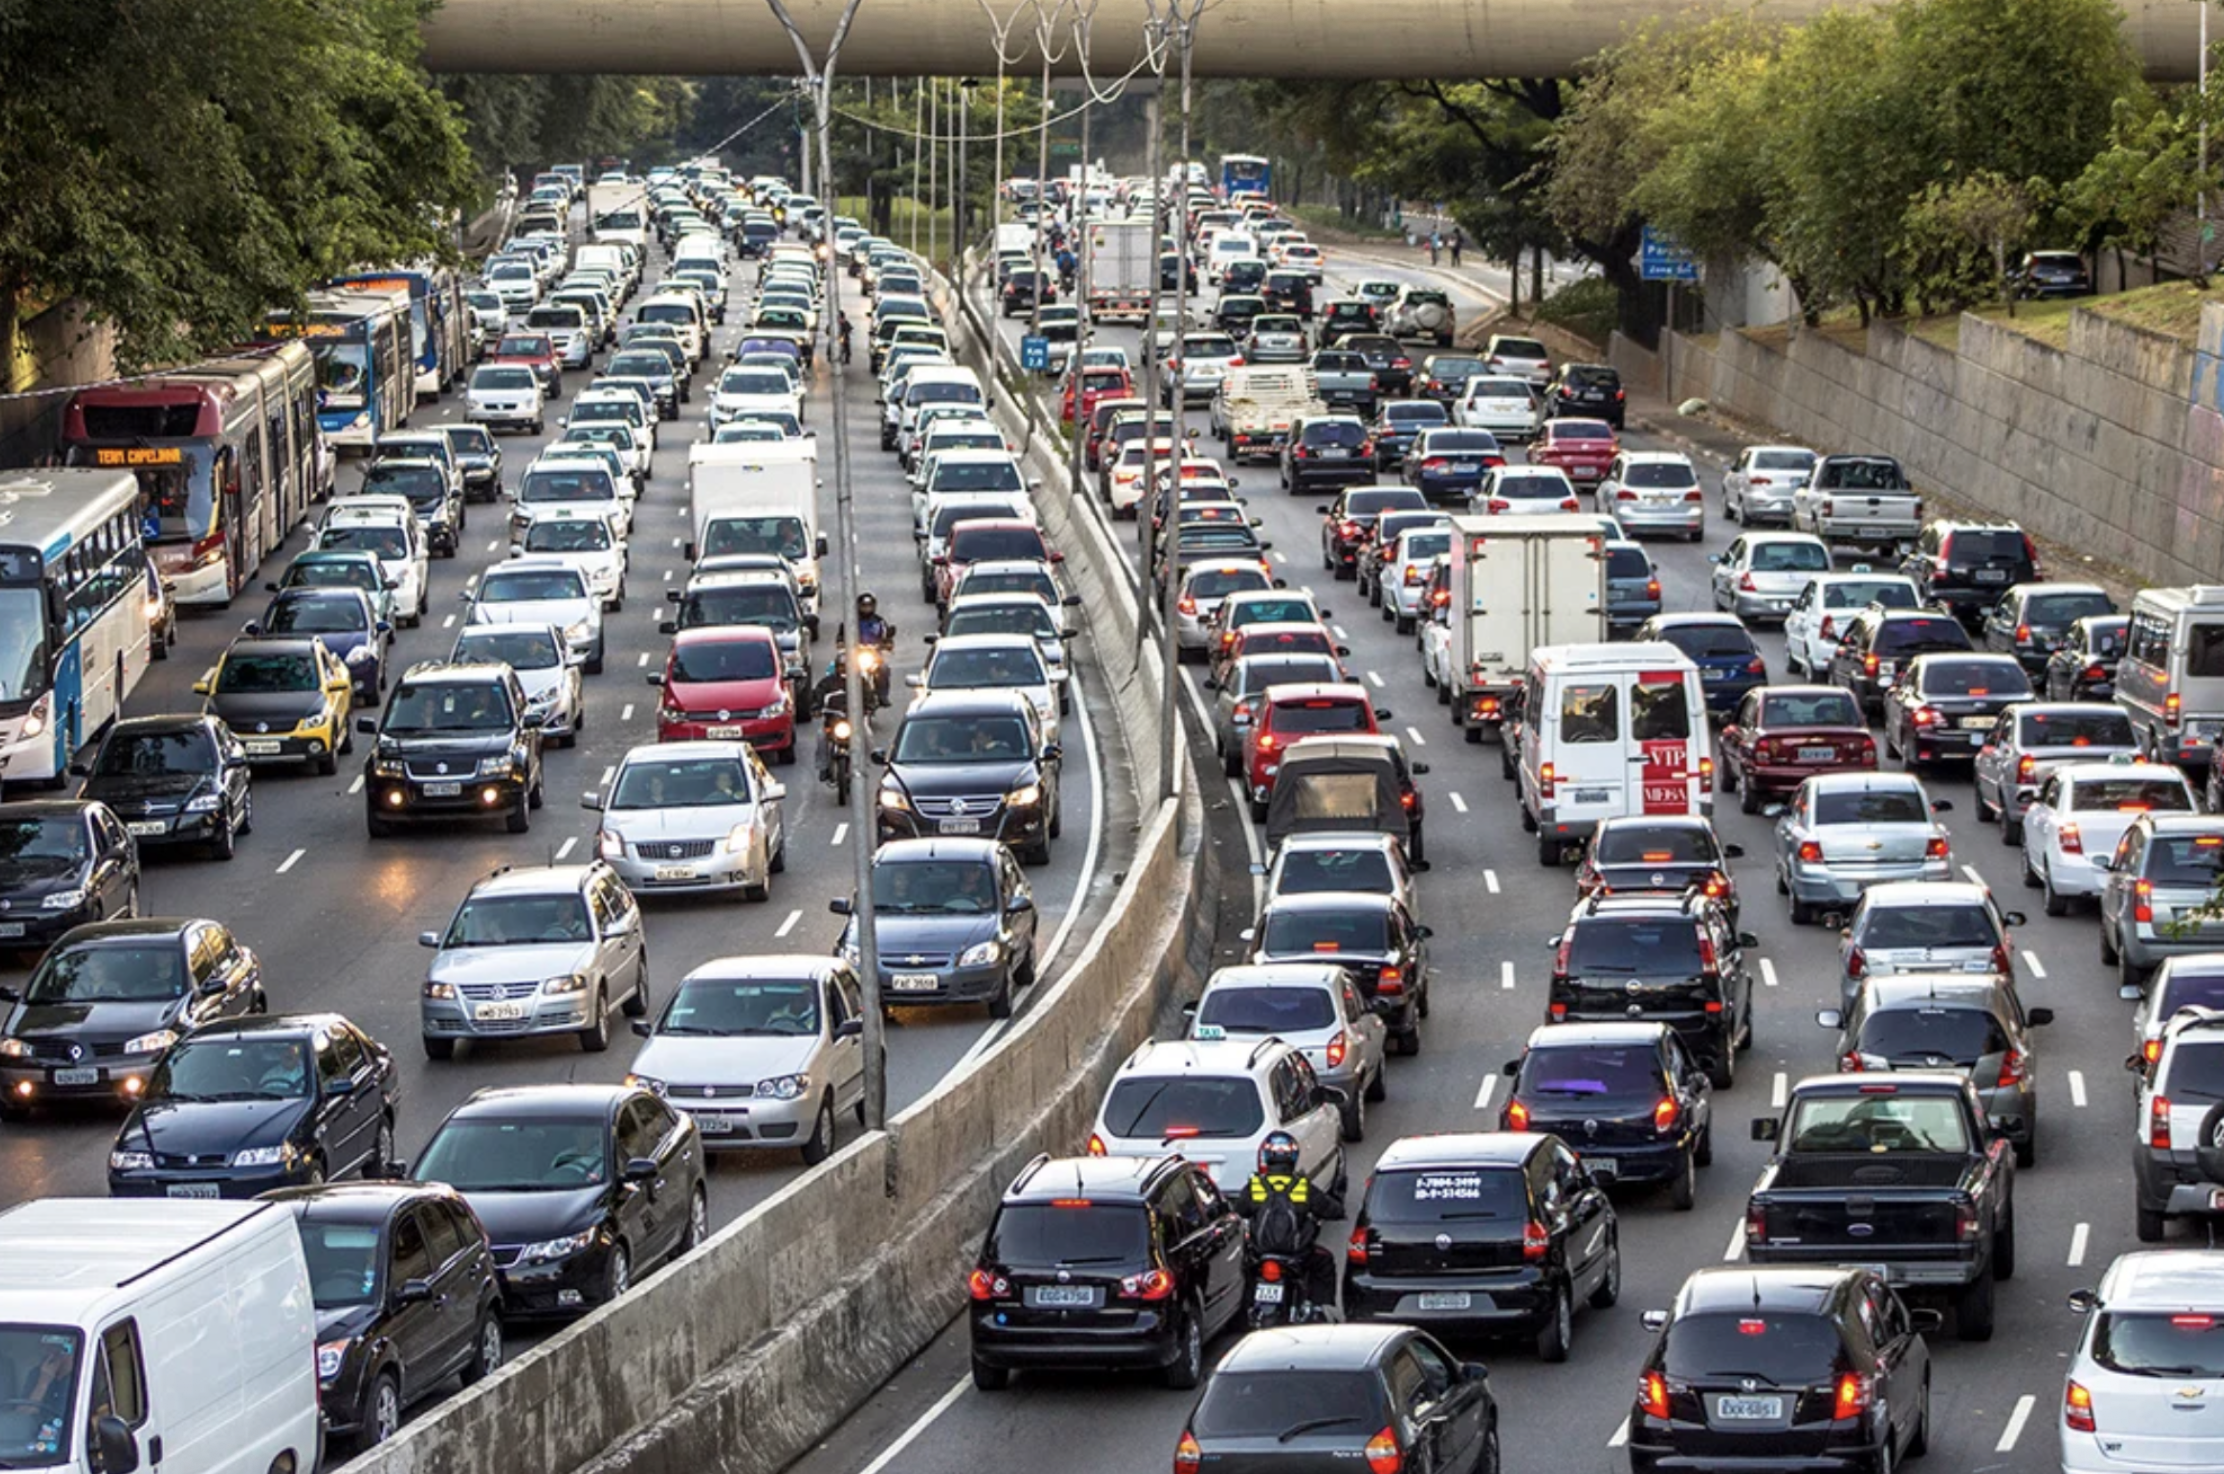
\includegraphics[width=0.6\textwidth]{assets/ch2/1.png}
    \caption{Camera Obscura principle.}
    \label{fig:camera_obscura}
\end{figure}

A simple setting for creating images on a white piece of paper is by projecting a shadow on it and, in the middle of the shadow, appears a picture of the scene in front of it. 

\begin{itemize}
    \item Leonardo da Vinci (1452-1519) was the first to describe the camera obscura in his notebooks.
    \item Johann Zahn (1685-1771) designed the first portable camera obscura in 1685.
    \item Joseph Nicephore Niepce (1765-1833) created the first permanent photograph in 1826 using a camera obscura.
\end{itemize}

\begin{minipage}{0.48\textwidth}
    From a geometrical point of view, the light rays of the object hit the film plane on different points, so we don't directly have the picture of the object. BUT, if we set a barrier in the middle, we have a one-to-one correspondence between the points of the object and the points of the film plane. That is why the pinhole camera works.
\end{minipage}
\hfill
\begin{minipage}{0.48\textwidth}
    \begin{figure}[H]
        \centering
        \includegraphics[width=0.8\textwidth]{assets/ch2/2.png}
        \caption{Pinhole camera principle.}
        \label{fig:pinhole_camera}
    \end{figure}
\end{minipage}

\begin{minipage}{0.48\textwidth}
    \begin{figure}[H]
        \centering
        \includegraphics[width=0.6\textwidth]{assets/ch2/3.png}
        \caption{Pinhole camera model.}
        \label{fig:pinhole_camera_model}
    \end{figure}
\end{minipage}
\hfill
\begin{minipage}{0.48\textwidth}
    \begin{itemize}
        \item The image is reversed upside-down and left-right;
        \item A \textit{virtual image} is formed in front of the camera.
    \end{itemize}
\end{minipage}

\paragraph{Perspective Projection} is composed by a \textit{principal plane}, parallel to the image plane and that contains the \textit{optical center ($C$)}. We then create the three axes, with the $Z$ one named \textit{principal axis}. 

\begin{figure}[H]
    \centering
    \includegraphics[width=\textwidth]{assets/ch2/4.png}
\end{figure}

Point $M$ is projected onto the image plane at point $M'$. By similarity of triangles, it follows that the 3D point $[X,Y,Z]^T$ is mapped to the point 
\[
[X',Y',Z']^T = \left[-\frac{f}{Z}X, -\frac{f}{Z}Y, -f\right]^T
\]
where $\frac{f}{Z}$ is the \textit{perspective scale factor}. Farther away objects (larger $Z$ appear smaller).

\paragraph{Weak Perspective} If the object is thin w.r.t. its distance from the camera, then the perspective scale factor is roughly constand:
\[
\frac{f}{Z_0 + \Delta Z} \approx \frac{f}{Z_0}
\]
Then, perspective projection can be approximated by a \textit{scaled orthographic projection}
\[
X' = -\frac{f}{Z_0}X, \quad Y' = -\frac{f}{Z_0}Y
\]
\begin{tipsblock}
    Rule of thumb due to Leonardo da Vinci: $\frac{\Delta Z}{Z_0} < \frac{1}{10}$
\end{tipsblock}

\begin{figure}[H]
    \centering
    \includegraphics[width=0.6\textwidth]{assets/ch2/5.png}
    \caption{Weak perspective projection.}
    \label{fig:weak_perspective}
\end{figure}

The \textbf{Aperture} is related to the amount of light that enters the camera. A larger aperture (smaller $f$-number) allows more light to enter, resulting in a brighter image. However, a larger aperture also reduces the depth of field, which is the range of distances within which objects appear sharp in the image.
\begin{itemize}
    \item \textbf{Pinhole too big} $\rightarrow$ many directions are averaged, blurring the image; sharp but dark image, because little light reaches the sensor;
    \item \textbf{Pinhole too small} $\rightarrow$ diffraction effects blur the image; brught but blurred image, because many directions are averaged.
\end{itemize}

\begin{figure}[H]
    \centering
    \includegraphics[width=0.8\textwidth]{assets/ch2/6.png}
    \caption{Aperture effects.}
    \label{fig:aperture_effects}
\end{figure}

Solution? \textbf{Lenses}!

\newpage
\subsection{Lenses}

A lens collects rays departing from the same points and focuses them onto the screen. There is a specific distance at which objects are in focus. Perspective projection is still valid within the thin lens assumption.

\begin{figure}[H]
    \centering
    \includegraphics[width=0.8\textwidth]{assets/ch2/7.png}
    \caption{Lens principle. The gray areas represent the set of rays originated from the object.}
    \label{fig:lens_principle}
\end{figure}

\begin{itemize}
    \item A \textit{thin lens} is composed of a single piece of glass with very low, equal curvature on both sides;
    \item Any ray that enters parallel to the axis on one side of the lens proceeds towards the \textbf{focal point $F$};
    \item Any ray that passes through the center of the lens $C$ does not change its direction;
    \item The distance $D$ from the center to the focal point is called \textbf{focal length $f$};
    \item The image $M'$ of $M$ can be found by intersecting two rays.
\end{itemize}

\begin{figure}[H]
    \centering
    \includegraphics[width=0.8\textwidth]{assets/ch2/8.png}
\end{figure}

Let's now try to use mathematical notation. Based on triangle similarity:
\[
\frac{Y'}{Y} = \frac{Z'}{Z}, \quad \frac{Y'}{Y} = \frac{Z' - D}{D}
\]
Thus, we get the \textbf{thin lens equation}, also known as the lensmaker's formula:
\[
\frac{1}{Z} + \frac{1}{Z'} = \frac{1}{D}
\]
which basically tells that points that are far away from the lens ($Z \to \infty$) are focused at the focal length ($Z' = D = f$).
Point $M$ is projected, when in focus, into the same position of a pinhole model having the optical center located in the lens center $C$.

\begin{minipage}{0.48\textwidth}
    \begin{itemize}
        \item Two points lying on opposite sides of the lens at distances that satisfy the thin lens equation are \textbf{conjugate points};
        \item In Figure \ref{fig:conjugate_points}, $A$ and $A'$ are conjugate;
        \item Parallel rays from infinity focus at distance $D$ from the lens;
        \item As a source of light rays moves closer to the lens, they focus further away on the other side;
        \item Rays originating from a point at a distance $D$ from the lens become parallel after passing throught the lens, i.e., they focus at infinity.
    \end{itemize}
\end{minipage}
\hfill
\begin{minipage}{0.48\textwidth}
    \begin{figure}[H]
        \centering
        \includegraphics[width=0.9\textwidth]{assets/ch2/9.png}
        \caption{Conjugate points.}
        \label{fig:conjugate_points}
    \end{figure}
\end{minipage}

